\section{Hardware}\label{sec:Hardware}
In diesem Kapitel werden die für den elektrischen Teil notwendigen Hardware-Komponenten detailliert beschrieben. Dabei umfasst es jegliche Komponenten, welche beim Betrieb einen elektrischen Anschluss besitzen wie beispielsweise Motor, Controller und die gesamte Energieversorgung. Da noch nicht alle Elemente bestimmt und ausgearbeitet wurden, fehlen einige Komponenten wie beispielsweise die Bremsschaltung mit entsprechendem Bremswiderstand oder evt. für den Betrieb notwendige Sensoren. Aus diesem Grund wird in diesem Kapitel lediglich die Auswahl von Motor und Controller, sowie eine erste Übersicht der Energieversorgung erläutert.


\subsection{Motor und Controller}\label{subsec:MotorController}
Um einen Gleitschirmpiloten in die Luft zu heben, muss der Motor über ein grosses Drehmoment und genügend Leistung verfügen. Aus der Literatur Gleitsegelschlepp \cite{Gleitsegelschlepp} ist ersichtlich, dass der Gleitschirmpilot mit einer Geschwindigkeit von bis zu 10m/s in Horizontalrichtung gezogen wird. Aus den Richtlinien, welche der deutsche Gleitschirmverband erlassen hat, ist wiederum ersichtlich, dass mit einer Zugkraft von bis zu $ 1000N $ bei Solopiloten und $ 1300N $ bei Tandempiloten gezogen werden darf \cite{WindenProtokoll}. Daraus lässt sich die maximale Leistung, welche das System auf den Gleitschirmpiloten ausüben darf, ausrechnen \cite{Kuchling}:


\begin{equation}
\centering
	P_{Seil}=F \cdot \nu=1300N \cdot 10m/s=13kW
\label{eq:LeistungSeil}
\end{equation}

$ P_{Seil} $\quad 	Leistung des Seils     \\
$ F $\qquad  Zugkraft des Seils    \\
$ \nu $\qquad  Geschwindigkeit     \\

Da es sich um ein reales System handelt und deswegen im Motor, in der Übertragung und Übersetzung Verluste auftreten, wird für die erste Handrechnung mit einem Gesamtwirkungsgrad des Systems von $80\%$ gerechnet.

\begin{equation}
\centering
	P_{Motor}=\frac{P_{Seil}}{\eta}=\frac{13kW}{0.8}=16.3kW
\label{eq:LeistungMotor}
\end{equation}

$ P_{Seil} $\quad 	Leistung des Seils     \\
$ P_{Motor} $  Leistung des Motors    \\
$ \eta $\qquad  Wirkungsgrad     \\

Dadurch dass sich zwischen den Schleppvorgängen jeweils eine Pause resultiert, muss diese Leistung nicht über einen längeren Zeitraum geleistet werden. Da Motoren durchaus kurzzeitig überlastet werden dürfen, darf die Nennleistung des Motors unter den 16.3kW liegen. Als Realisierungsmöglichkeiten kamen somit lediglich Wechselstrommotoren mit Wechselrichter, DC-Motoren oder Brushless DC (auch BLDC) Motoren in Frage. Eine Auswahl an Motoren mit deren Controller ist im Anhang \ref{appsec:Motoren} aufgelistet.\\
Damit die Schleppwinde auf dem Markt wettbewerbsfähig ist, muss diese sowohl günstig sein, als auch alle elektrischen und mechanischen Anforderungen gänzlich erfüllen. Aufgrund des besten Preis-/ Leistungsverhältnissen und der hohen Nennleistung mit $ 13kW $, fiel der Entscheid gemeinsam mit dem Auftraggeber auf den BLDC-Motor des Herstellers $ Goldenmotors $. Da dieser Motor in verschiedenen Betriebsspannungen ausgeführt wird ($ 48V $, $ 72V $ und $ 96V $), war aufgrund der Verlustleistung (welche sich durch den Strom im Quadrat berechnet), ein möglichst kleinerer Strom und somit eine hohe Spannung anstrebenswert. Da die Energieversorgung durch Bleiakkus realisiert wird und diese eine hohe Leerlaufspannung aufweisen (geladen 14.4V statt 12V pro Batterie), wird bei den notwendigen 96V eine Spannung von rund 116V erreicht, was nach wie vor im Kleinspannungsbereich liegt. Aus diesem Grund wurde das 96V Modell ausgewählt. Durch diesen Entscheid können sowohl beim Versuchsaufbau als auch bei der finalen Konstruktion kleinere Leiterquerschnitte gefahren werden, welches wiederum geringere Materialkosten zur Folge hat. Weiter konnte zwischen einem luftgekühlten und wassergekühlten Modell entschieden werden, wobei aufgrund des aufwändigen Aufbaus einer Wasserkühlung, der Entschied auf eine Luftkühlung fiel.  

%Damit die Verlustleistung so klein wie möglich gehalten werden kann, ist es notwendig den Strom so tief wie möglich zu halten. Da dieser Motor in verschiedenen Betriebsspannungen ausgeführt wird ($ 48V $, $ 72V $ und $ 96V $), wurde die Variante mit der höchsten Spannung ausgewählt. 

\subsection{Energieversorgung}\label{subsec:Energieversorgung}

Für den Betrieb der Einzugswinde wird das gesamte System von einer Batterie gespiessen. Wie im vorhergehenden Abschnitt \ref{subsec:MotorController} beschrieben, wurde ein Motor mit 96V Nennspannung ausgewählt. Aus diesem Grund ist es notwendig, Batterien mit derselben Versorgungsspannung zu verwenden. Trotz der steilen Entwicklungskurve von Li-Io-Akku sind diese im Vergleich zu kommerziellen Bleiakkus heikler in der Handhabung (Ladeschaltung mit Zellenausgleich, Überlade- und Tiefentladeüberwachung notwendig) und vor allem teurer. Es muss berücksichtigt werden, dass auch bei Bleiakkus zwischen zwei Typen unterschieden wird. Zum einen gibt es Starterbatterien (hohe Anlaufströme, kurze Laufzeit) und zum anderen zyklenfeste Bleiakkus (lange Laufzeit, ausgelegt für viele Lade-/ Entladevorgänge).

Um einen Überblick zu erhalten, befinden sich im Anhang \ref{appsec:Batterie} zwei Tabellen mit einigen Modellen von jedem Typen. Diese werden jeweils in den elektrischen Klassifizierungen (Typ, Spannung, Kapazität), wie auch weiteren Merkmalen (wie Gewicht, Preis, Anzahl Starts) mit einander verglichen. Die zyklenfesten Batterien wurden zusätzlich mit den vom Hersteller angegebenen Zyklenfestigkeit und den jeweiligen Innenwiderständen ergänzt. Der Innenwiderstand wichtig, weil bei hohen Strömen (gemäss dem Ohmschen Gesetz) eine Spannung über den Batterien abfällt. Daher gilt: Umso grösser der Innenwiderstand, desto grösser die abfallende Spannung über den Batterien, wodurch eine kleinere Spannung an den Motor gelangt.
Als Referenzwert zur Kapazität, wurden die Anzahl möglichen Starts in Abhängigkeit zur Kapazität mittels den Formeln \ref{eq:EnergieStart} bis \ref{eq:AnzahlStarts} berechnet. Dafür wurden nachfolgende Annahmen getroffen. 

\begin{table}[H]
	\centering
	\begin{tabular}{C{5cm} C{2.5cm} C{2cm}}
		\multicolumn{3}{c}{}\\
	{Beschreibung} & {Index} & {Wert} \\ \hline
	Zugkraft    &   $ F_{Zug} $    & $10 kN$   \\
	Geschwindigkeit    &   $ v $    & $10 m/s$   \\
	Startzeit    &   $ t $   & $120 s$   \\
	Gesamtwirkungsgrad    &  $ \eta_{tot} $    & $80\%$   \\
	Auslastung    &  $ \theta $   & $80\%$  \\
	Batterieausnutzung    &  $ \kappa $    & $60\%$   \\
	Gesamte Batteriekapazität   &   $ Q $    &   \\
	Gesamte Batteriespannung    &   $ U_{Bat,tot} $    &   \\
	Energie für Startvorgang    &   $ W_{Start} $    &   \\
	Gesamtenergie von Batterie   &   $ W_{Bat} $    &   \\
	Anzahl Starts    &   $ n $    &    \\	
	\end{tabular}
	\caption{Annahmen für Berechnung}
	\label{tab:BerechnungAnzahlStart}
\end{table}

\begin{equation}
\centering
	W_{Start}=\frac{F_{Zug}\cdot v \cdot t}{\eta_{tot}\cdot 3600}\cdot \theta
\label{eq:EnergieStart}
\end{equation}

\begin{equation}
\centering
	W_{Bat}=U_{Bat,tot}\cdot Q \cdot \kappa
\label{eq:EnergieBatterie}
\end{equation}

\begin{equation}
\centering
	n=\frac{W_{Start}}{W_{Bat}}
\label{eq:AnzahlStarts}
\end{equation}


Werden die aufgelisteten Batterien untereinander verglichen, so ist die Batterie des Herstellers $Long$ durch das Preis/Leistungsverhältnis und seine Zyklenfestigkeit augenfällig. Deren Entladeverhalten bei unterschiedlichen Strömen (\ref{fig:EntladeStrom}) und dessen Entladeverhalten bei unterschiedlicher Entladung (\ref{fig:EntladeKapazität}) ist nachfolgend ersichtlich. 


\begin{figure}[H]
	\centering
	\begin{minipage}[h]{.48\linewidth} % [b] => Ausrichtung an \caption
		\centering
		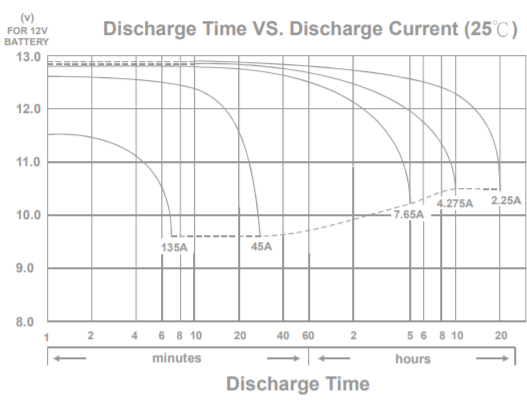
\includegraphics[width=\linewidth]{LongEntladeStrom.png}
		\caption[Batterie Entladeverhalten Strom]{Entladeverhalten Strom}
		\label{fig:EntladeStrom}
	\end{minipage}
	\quad % Abstand zwischen Bilder
	\begin{minipage}[h]{.48\linewidth} % [b] => Ausrichtung an \caption
		\centering
		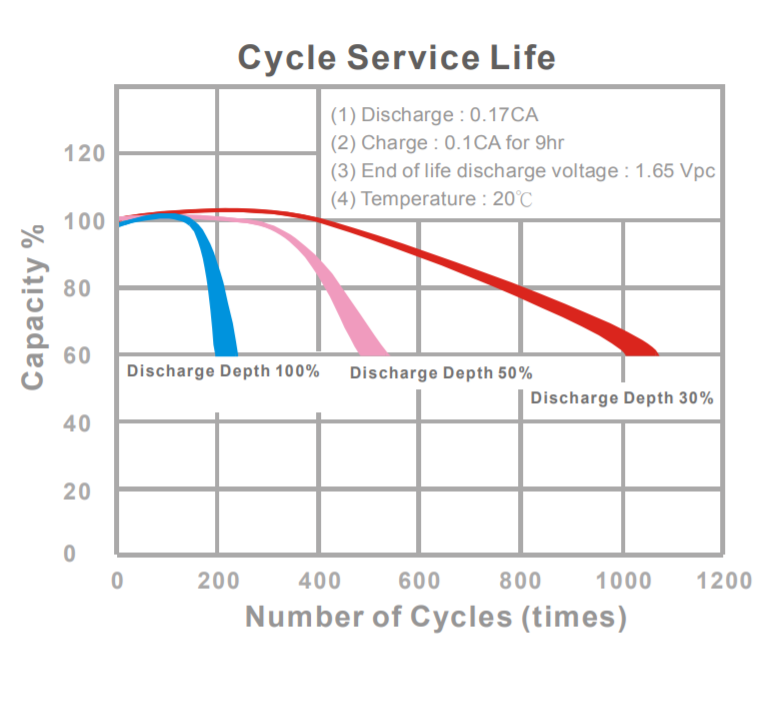
\includegraphics[width=\linewidth]{LongEntladeKapa.png}
		\caption[Batterie Entladeverhalten Kapazität]{Entladeverhalten Kapazität}
		\label{fig:EntladeKapazität}
	\end{minipage}
\end{figure}

In der Abbildung \ref{fig:EntladeStrom} ist unschwer zu erkennen, dass ab einer Spannung von rund 10.5V kaum Kapazität aus der Batterie herausgeholt werden kann und die Spannung stark abnimmt. Welche Auswirkung die Intensität eines Entladezyklus hat, ist in der Abbildung \ref{fig:EntladeKapazität} ersichtlich. Wird die Batterie mit 100\% entladen, besitzt sie ab 200 Zyklen lediglich noch 60\% der Nennkapazität. Betrachtet man das kleine Kästchen innerhalb der Abbildung \ref{fig:EntladeKapazität}, sind die Bedingungen der Messung ersichtlich. Es gilt zu beachten, dass die Temperatur beim Entladeversuch optimal auf 20°C gehalten wird. Der Entlade- sowie Ladestrom wird in den Datenblättern üblicherweise als CA-Wert (Cranking Amperes) angegeben und ist eine Angabe, welche sich auf die Kapazität der Batterie stützt. Der Strom berechnet sich gemäss nachfolgender Formel \ref{eq:CA}.

\begin{equation}
\centering
I=CA \cdot Q
\label{eq:CA}
\end{equation}
$ CA $\quad 	Cracking Amperes      \\
$ Q $\qquad  Kapazität Batterie     \\

Betrachtet man Abbildung \ref{fig:EntladeKapazität}, so ist ersichtlich, dass der Strom bei der Entladung 7.65A und beim Ladevorgang 4.5A beträgt.
Es gilt zu beachten, dass die minimale Zellenspannung (End of life discharge voltage) von 1.65V auf keinen Fall unterschritten wird, da dies ansonsten zur Zerstörung der Zelle führt. Da eine Batterieeinheit sechs Zellen besitzt, resultiert daraus eine minimale Spannung von 9.9V. Diese Berechnungen lassen sich auch auf andere Blei-Vlies-Akkumulatoren übertragen und weichen lediglich durch die Zyklenfestigkeit und einem anderen CA-Wert ab.